\documentclass[twocolumn, 10pt]{article}
\setlength\textwidth{6.875in}
\setlength\textheight{8.875in}
% set both margins to 2.5 pc
\setlength{\oddsidemargin}{-0.1875in}% 1 - (8.5 - 6.875)/2
\setlength{\evensidemargin}{-0.1875in}
\setlength{\marginparwidth}{0pc}
\setlength{\marginparsep}{0pc}%
\setlength{\topmargin}{0in} \setlength{\headheight}{0pt}
\setlength{\headsep}{0pt}
\setlength{\footskip}{37pt}%
%\setlength{\columnsep}{0.3125in}
%\setlength{\columnwidth}{3.28125in}% (6.875 - 0.3125)/2 = 3.28125in
\setlength{\parindent}{1pc}
\newcommand{\myMargin}{1.00in}
\usepackage[top=\myMargin, left=\myMargin, right=\myMargin, bottom=\myMargin, nohead]{geometry}
\usepackage{epsfig,graphicx}
\usepackage{palatino}
\usepackage{fancybox}
\usepackage{hyperref}
\usepackage[procnames]{listings}

% "define" Scala
\usepackage[T1]{fontenc}  
\usepackage[scaled=0.82]{beramono}  
\usepackage{microtype} 

\sbox0{\small\ttfamily A}
\edef\mybasewidth{\the\wd0 }

\lstdefinelanguage{scala}{
  morekeywords={abstract,case,catch,class,def,%
    do,else,extends,false,final,finally,%
    for,if,implicit,import,match,mixin,%
    new,null,object,override,package,%
    private,protected,requires,return,sealed,%
    super,this,throw,trait,true,try,%
    type,val,var,while,with,yield},
  sensitive=true,
  morecomment=[l]{//},
  morecomment=[n]{/*}{*/},
  morestring=[b]",
  morestring=[b]',
  morestring=[b]"""
}

\usepackage{color}
\definecolor{dkgreen}{rgb}{0,0.6,0}
\definecolor{gray}{rgb}{0.5,0.5,0.5}
\definecolor{mauve}{rgb}{0.58,0,0.82}

% Default settings for code listings
\lstset{frame=tb,
  language=scala,
  aboveskip=3mm,
  belowskip=3mm,
  showstringspaces=false,
  columns=fixed, % basewidth=\mybasewidth,
  basicstyle={\small\ttfamily},
  numbers=none,
  numberstyle=\footnotesize\color{gray},
  % identifierstyle=\color{red},
  keywordstyle=\color{blue},
  commentstyle=\color{dkgreen},
  stringstyle=\color{mauve},
  frame=single,
  breaklines=true,
  breakatwhitespace=true,
  procnamekeys={def, val, var, class, trait, object, extends},
  procnamestyle=\ttfamily\color{red},
  tabsize=2
}

\lstnewenvironment{scala}
{\lstset{language=scala}}
{}
\lstnewenvironment{cpp}
{\lstset{language=C++}}
{}
\lstnewenvironment{bash}
{\lstset{language=bash}}
{}
\lstnewenvironment{verilog}
{\lstset{language=verilog}}
{}



\lstset{basicstyle={\footnotesize\ttfamily}}

\newenvironment{commentary}
{ \vspace{-0.1in}
  \begin{quotation}
  \noindent
  \small \em
  \rule{\linewidth}{1pt}\\
}
{
  \end{quotation}
}

\title{Getting Started: Tutorial 01 - The Basics}
\author{Jonathan Bachrach, Vincent Lee \\
EECS Department, UC Berkeley\\
{\tt  \{jrb\}@eecs.berkeley.edu}
}
\date{\today}

\newenvironment{example}{\VerbatimEnvironment\begin{footnotesize}\begin{Verbatim}}{\end{Verbatim}\end{footnotesize}}
\newcommand{\kode}[1]{\begin{footnotesize}{\tt #1}\end{footnotesize}}

\def\code#1{{\tt #1}}

\def\note#1{\noindent{\bf [Note: #1]}}
%\def\note#1{}

\begin{document}
\maketitle{}

\section{Introduction}

Ths document is intended to get you started with basic constructs in Chisel with a series of basic examples from the Chisel tutorial.  The tutorial is broken into small modules each of which highlights some of the powerful features of Chisel. This tutorial also contains exercises which will walk you through the basics and assumes knowledge of basic digital systems design.

\subsection{Acquiring the Tutorial Files}

To get the files required for this tutorial, you will need to have Git installed on your machine. Change directory to the place you would like to place your Chisel files (let's call this \verb+$DIR+ from now on) and get the tutorial files with:

\begin{bash}
git clone https://github.com/ucb-bar/chisel-tutorial.git
\end{bash}

This will clone the Chisel tutorial files onto your machine. If you cloned the repository into \verb+$DIR+ then your copy of the Chisel Tutorial repository will then be in \verb+$DIR/chisel-tutorial+.  Define this as a variable in your bash environment:

\subsection{The Chisel Directory Structure}

Once you have acquired the tutorial files you should see the following Chisel tutorial directory structure under \verb+$DIR+:

\begin{bash}
chisel-tutorial/  
  Makefile
  examples/   # Contains chisel examples
    Makefile  
    build.sbt # Contains project file
    Accumulator.scala ...
    emulator/ # Contains C++ simulation build products
    verilog/  # Contains Verilog build products
  problems/   # Contains skeletal files for tutorial problems
    Makefile
    build.sbt # Contains project file
    Counter.scala ...
    emulator/ # Contains C++ simulation build products
    verilog/  # Contains Verilog build products
  solutions/  # Contains solutions to problems
    Makefile
    build.sbt # Contains project file
    Counter.scala ...
    emulator/ # Contains C++ simulation build products
    verilog/  # Contains Verilog build products
\end{bash}

The \verb+src/+ directory contains all of your Chisel source files. For our tutorial it contains the files that you will be modifying under \verb+problems/+ while the \verb+solutions/+ folder contains the reference implementations for each of the problems.  Finally, \verb+examples/+ contains source to the complete examples given in this tutorial.

The \verb+emulator/+ directories contain the generated C++ files required to simulate the Chisel source files. We will explain more about the simulation directories later.

The \verb+verilog/+ directories contain the generated Verilog files corresponding to your Chisel sources. Recall that Chisel is a hardware constructing language so this directory is where all of the magic occurs and produces FPGA or ASIC Verilog.

Finally, the \verb+build.sbt+ files contain the build configuration information used to specify what version of Chisel to make your project with.

\section{Running Your First Chisel Build}

In this section, we explain how to run your first build to explore what Chisel has to offer. We will go through a simple example for a GCD module and familiarize ourselves with the source files, simulation, and Verilog generation. More comprehensive details will follow in subsequent sections of the tutorial.

\subsection{The Chisel Source Code}

Now that you are more familiar with what your Chisel directory structure contains, let's start by exploring one of the Chisel files. Change directory into the \verb+examples/+ directory and open up the \verb+GCD.scala+ file with your favorite text editor. 

You will notice that file is already filled out for you to perform the well known GCD algorithm and should look like:

\begin{scala}
package TutorialExamples

import Chisel._
import scala.collection.mutable.HashMap

class GCD extends Module {
  val io = new Bundle {
    val a  = UInt(INPUT,  16)
    val b  = UInt(INPUT,  16)
    val e  = Bool(INPUT)
    val z  = UInt(OUTPUT, 16)
    val v  = Bool(OUTPUT)
  }
  val x  = Reg(UInt())
  val y  = Reg(UInt())
  when   (x > y) { x := x - y } 
  unless (x > y) { y := y - x }
  when (io.e) { x := io.a; y := io.b }
  io.z := x
  io.v := y === UInt(0)
} ...
\end{scala}

The first thing you will notice is the \verb+import Chisel._+ declaration; this imports the Chisel library files that allow us to leverage Scala as a hardware construction language. After the import declarations you will see the Scala class definition for the Chisel component you are implementing. You can think of this as almost the same thing as a module declaration in Verilog.

Next we see the I/O specification for this component in the \verb+val io = new Bundle{...}+ definition. You will notice that the bundle takes several arguments as part of its construction, each with a specified type (UInt, Bool, etc.), a direction (either INPUT or OUTPUT), and a bit width. If a bit width is not specified, Chisel will infer the appropriate bit width for you (in this case default to 1). The \verb+io+ Bundle is essentially a constructor for the component that we are constructing.

The next section of code performs the actual GCD computation for the module. The register declarations for \verb+x+ and \verb+y+ tell Chisel to treat \verb+x+ and \verb+y+ as a register of type UInt(). 

\begin{scala}
val x  = Reg(UInt())  // declares x as UInt register
val y  = Reg(UInt())  // declares y as UInt register
\end{scala}

The \verb+when+ statement tells Chisel to perform the operation on a positive clock edge if the condition is true, treating the left hand assignments as synchronous. This is similar to how Verilog uses \verb+always @ (posedge clk)+ to specify synchronous logic.

Finally we see the output assignments for the computation for \verb+io.z+ and \verb+io.v+. One particular thing to notice is that, we do not have to specify the width of \verb+x+ and \verb+y+ in this example. This is because Chisel does the bit width inference for you and sets these values to their appropriate widths based on the computation they are storing.

\subsection{Running the Chisel Simulation}

Now that we are familiar with the Chisel code for the \verb+GCD.scala+ file, let's try to simulate it by generating the C++ models. Change directory into the \verb+$DIR/problems/+ directory. Here you will see one lonely Makefile which we will call with:

\begin{bash}
make GCD
\end{bash}

This will fire off the Chisel emulator that will run the simulation for the component defined in \verb+GCD.scala+. If the simulation succeeds, you should see some debug output followed by:
\begin{bash}
PASSED
[success] Total time: 2 s, completed Feb 28, 2013 8:14:37 PM
\end{bash}

The debug output is generated by the test harness which composes the second half of the GCD.scala file. We will talk about this more later. In addition to the debug output, the build also creates C++ models which can be used to simulate and debug more complicated designs.

\subsection{Generating the Verilog}

One of the most powerful features of Chisel is its ability to generate FPGA and ASIC Verilog from the Scala sources that you construct. To do this, change directory into the \verb+$DIR/problems/verilog/+ directory and again run:
\begin{bash}
make GCD.v
\end{bash}
This will start the Verilog generation for the GCD Chisel file. When the Verilog generation finishes, you should see a [success] message similar to the one you saw in the emulator and a new \verb+GCD.v+ file. If you open up \verb+GCD.v+, you will find that Chisel has compiled \verb+GCD.scala+ into its equivalent Verilog source.

You will find that the Chisel compiler has generated an equivalent Verilog module that performs the GCD computation.

The Verilog source is roughly divided into three parts:
\begin{enumerate}
\item Module declaration with input and outputs
\item Temporary wire and register declaration used for holding intermediate values
\item Register assignments in \verb+always @ (posedge clk)+
\end{enumerate}

\section{Combinational Logic}

\subsection{The Scala Node: Declaring Wires}

Constructing combinational logic blocks in Chisel is fairly straightforward; when you declare a \verb+val+ in Scala, it creates a node that represents the data that it is assigned to. As long as the value is not assigned to be a register type (explained later), this tells the Chisel compiler to treat the value as wire. Thus any number of these values can be connected and manipulated to produce the value that we want.

Suppose we want to construct a single full adder. A full adder takes two inputs \verb+a+ and \verb+b+, and a carry in \verb+cin+ and produces a \verb+sum+ and carry out \verb+cout+. The Chisel source code for our full adder will look something like:

\begin{scala}
class FullAdder extends Module {
  val io = new Bundle {
    val a    = UInt(INPUT, 1)
    val b    = UInt(INPUT, 1)
    val cin  = UInt(INPUT, 1)
    val sum  = UInt(OUTPUT, 1)
    val cout = UInt(OUTPUT, 1)
  }
  //Generate the sum
  val a_xor_b = io.a ^ io.b
  io.sum := a_xor_b ^ io.cin
  //Generate the carry
  val a_and_b = io.a & io.b
  val b_and_cin = io.b & io.cin
  val a_and_cin = io.a & io.cin
  io.cout := a_and_b | b_and_cin | a_and_cin
}
\end{scala}

You will notice that in order to access the input values from the \verb+io+ bundle, you need to first reference \verb+io+ since the input and output values belong to the \verb+io+ bundle. The |, \&, and \^\ operators correspond to bitwise OR, AND, and XOR operations respectively.

The corresponding wires for each of these values is shown below:

\begin{figure}[ht!]
\centering
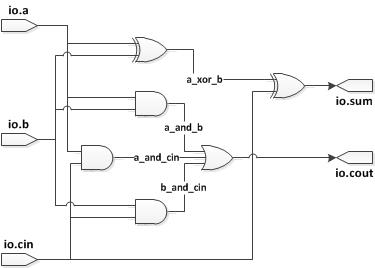
\includegraphics[width=80mm]{Full_Adder.jpg}
\caption{Full Adder Circuit}
\end{figure}

You will notice that each \verb+val+ corresponds to exactly one of the wires.

\subsection{Bit Width Inference}

If you don't explicitly specify the width of a value in Chisel, the Chisel compiler will infer the bit width for you based on the inputs that define the value. Notice in the \verb+FullAdder+ definition, the widths for \verb+a_xor_b, a_and_b, b_and_cin,+ and \verb+a_and_cin+ are never specified anywhere. However, based on how the input is computed, Chisel will correctly infer each of these values are one bit wide since each of their inputs are the results of bitwise operations applied to one bit operands.

A quick inspection of the generated Verilog shows these values are indeed one bit wide:

\begin{bash}
module FullAdder(
    input  io_a,
    input  io_b,
    input  io_cin,
    output io_sum,
    output io_cout);

  wire T0;
  wire a_and_cin;
  wire T1;
  wire b_and_cin;
  wire a_and_b;
  wire T2;
  wire a_xor_b;

  assign io_cout = T0;
  assign T0 = T1 | a_and_cin;
  assign a_and_cin = io_a & io_cin;
  assign T1 = a_and_b | b_and_cin;
  assign b_and_cin = io_b & io_cin;
  assign a_and_b = io_a & io_b;
  assign io_sum = T2;
  assign T2 = a_xor_b ^ io_cin;
  assign a_xor_b = io_a ^ io_b;
endmodule
\end{bash}

Suppose we change the widths of the \verb+FullAdder+ to be 2 bits wide each instead such that the Chisel source now looks like:

\begin{scala}
class FullAdder extends Module {
  val io = new Bundle {
    val a    = UInt(INPUT, 2)
    val b    = UInt(INPUT, 2)
    val cin  = UInt(INPUT, 2)
    val sum  = UInt(OUTPUT, 2)
    val cout = UInt(OUTPUT, 2)
  }
  // Generate the sum
  val a_xor_b = io.a ^ io.b
  io.sum := a_xor_b ^ io.cin
  // Generate the carry
  val a_and_b = io.a & io.b
  val b_and_cin = io.b & io.cin
  val a_and_cin = io.a & io.cin
  io.cout := a_and_b | b_and_cin | a_and_cin
\end{scala}

As a result, the Chisel compiler should infer each of the intermediate values \verb+a_xor_b, a_and_b, b_and_cin,+ and \verb+a_and_cin+ are two bits wide. An inspection of the Verilog code correctly shows that Chisel inferred each of the intermediate wires in the calculation to be 2 bits wide.

\begin{bash}
module FullAdder(
    input [1:0] io_a,
    input [1:0] io_b,
    input [1:0] io_cin,
    output[1:0] io_sum,
    output[1:0] io_cout);

  wire[1:0] T0;
  wire[1:0] a_and_cin;
  wire[1:0] T1;
  wire[1:0] b_and_cin;
  wire[1:0] a_and_b;
  wire[1:0] T2;
  wire[1:0] a_xor_b;

  assign io_cout = T0;
  assign T0 = T1 | a_and_cin;
  assign a_and_cin = io_a & io_cin;
  assign T1 = a_and_b | b_and_cin;
  assign b_and_cin = io_b & io_cin;
  assign a_and_b = io_a & io_b;
  assign io_sum = T2;
  assign T2 = a_xor_b ^ io_cin;
  assign a_xor_b = io_a ^ io_b;
endmodule
\end{bash}

\section{Using Registers}

Unlike Verilog, specifying a register in Chisel tells the compiler to actually generate a positive edge triggered register. In this section we explore how to instantiate registers in Chisel by constructing a shift register.

In Chisel, when you instantiate a register there are several ways to specify the connection of the input to a register. As shown in the GCD example, you can "declare" the register and assign what it's input is connected to in a \verb+when...+ block or you can simply pass the value that the register is clocking as a parameter to the register.

If you choose to pass a next value to the register on construction using the \verb+next+ named parameter, it will clock the new value every cycle unconditionally:

\begin{scala}
// Clock the new register value on every cycle
val y = io.x
val z = Reg(next = y)
\end{scala}

If we only want to update if certain conditions are met we use a \verb+when+ block to indicate that the registers are only updated when the condition is satisfied:

\begin{scala}
//Clock the new register value when the condition a > b
val x = Reg(UInt())
when (a > b) { x := y }
.elsewhen ( b > a) {x := z}
.otherwise { x := w}
\end{scala}

It is important to note that when using the conditional method that the values getting assigned to the input of the register matches the type and bitwidth of the register you declared. In the unconditional register assignment, you do not need to do this as Chisel will infer the type and width from the type and width of the input value.

The following sections show how these can be used to construct a shift register.

\subsection{Unconditional Register Update}

Suppose we want to construct a basic 4 bit shift register that takes a serial input \verb+in+ and generates a serial output \verb+out+. For this first example we won't worry about a parallel load signal and will assume the shift register is always enabled. We also will forget about the register reset signal.

If we instantiate and connect each of these 4 registers explicitly, our Chisel code will look something like:

\begin{scala}
class ShiftRegister extends Module {
  val io = new Bundle {
    val in  = UInt(INPUT, 1)
    val out = UInt(OUTPUT, 1)
  }
  val r0 = Reg(next = io.in)
  val r1 = Reg(next = r0)
  val r2 = Reg(next = r1)
  val r3 = Reg(next = r2)
  io.out := r3
}
\end{scala}

If we take a look at the generated Verilog, we will see that Chisel did indeed map our design to a shift register. One thing to notice is that the clock signal and reset signals are implicitly attached to our design.

\begin{bash}
module ShiftRegister(input clk, input reset,
    input  io_in,
    output io_out);

  reg[0:0] r3;
  reg[0:0] r2;
  reg[0:0] r1;
  reg[0:0] r0;

  assign io_out = r3;
  always @(posedge clk) begin
    r3 <= r2;
    r2 <= r1;
    r1 <= r0;
    r0 <= io_in;
  end
endmodule
\end{bash}

\subsection{Conditional Register Update}

As mentioned earlier, Chisel allows you to conditionally update a register (use an enable signal) using the \verb+when+, \verb+.elsewhen+, \verb+.otherwise+ block. Suppose we add an enable signal to our shift register, that allows us to control whether data is shift in and out on a given cycle depending on an \verb+enable+ input signal. The new shift register now looks like:

\begin{scala}
class ShiftRegister extends Module {
  val io = new Bundle {
    val in     = UInt(INPUT, 1)
    val enable = UInt(INPUT, 1)
    val out    = UInt(OUTPUT, 1)
  }

  val r0 = Reg(UInt())
  val r1 = Reg(UInt())
  val r2 = Reg(UInt())
  val r3 = Reg(UInt())

  when (io.enable) {
    r0 := io.in
    r1 := r0
    r2 := r1
    r3 := r2
  }
  io.out := r3
}
\end{scala}

Notice that it is not necessary to specify an \verb+.otherwise+ condition as Chisel will correctly infer that the old register value should be preserved otherwise.

\subsection{Register Reset}

Chisel allows you to specify a synchronous reset to a certain value by specifying an additional parameter when you first declare them. In our shift register, let's add a reset capability that resets all the register values to zero synchronously. To do this we need to provide our register declarations a little more information using the \verb+init+ parameter with what value we want on a synchronous reset:

\begin{scala}
class ShiftRegister extends Module {
  val io = new Bundle {
    val in     = UInt(INPUT, 1)
    val enable = UInt(INPUT, 1)
    val out    = UInt(OUTPUT, 1)
  }
  // Register reset to zero
  val r0 = Reg(init = UInt(0, width = 1))
  val r1 = Reg(init = UInt(0, width = 1))
  val r2 = Reg(init = UInt(0, width = 1))
  val r3 = Reg(init = UInt(0, width = 1))
  when (io.enable) {
    r0 := io.in
    r1 := r0
    r2 := r1
    r3 := r2
  }
  io.out := r3
}
\end{scala}

Notice that reset value can actually be any value, simply replace the zeros and width to appropriate values.

Chisel also has an implict global \verb+reset+ signal that you can use in a \verb+when+ block. The reset signal is conveniently called \verb+reset+ and does not have to be declared. The shift register using this implict global reset now looks like:

\begin{scala}
class ShiftRegister extends Module {
  val io = new Bundle {
    val in     = UInt(INPUT, 1)
    val enable = UInt(INPUT, 1)
    val out    = UInt(OUTPUT, 1)
  }
  val r0 = Reg(UInt())
  val r1 = Reg(UInt())
  val r2 = Reg(UInt())
  val r3 = Reg(UInt())
  when(reset) {
    r0 := UInt(0)
    r1 := UInt(0)
    r2 := UInt(0)
    r3 := UInt(0)
  } .elsewhen(io.enable) {
    r0 := io.in
    r1 := r0
    r2 := r1
    r3 := r2
  }
  io.out := r3
}
\end{scala}

This will generate slightly different looking Verilog source code but will still function the same as the previous implementation of the shift register with reset.

%\section{Tutorial Exercises}

%The following exercises can be found in your \verb+\$DIR/chisel-tutorial/src/problems/+ folder. You will find that some parts of the tutorial files have been completed for you and the section that you need to will need to complete is indicated in the file. The solutions to each of these exercises can be found in the \verb+\$DIR/chisel-tutorial/src/solutions/+ folder.

%\subsection{Creating a Two Input Multiplexor}
%
%<IS THIS EVEN A GOOD IDEA BECAUSE THEY DON'T REALLY KNOW ANYTHING YET>
%
%\subsection{Creating a Simple FIFO}
%
%<IS THIS EVEN A GOOD IDEA BECAUSE THEY DON'T REALLY KNOW ANYTHING YET>
%
\end{document}
